\documentclass{beamer}
\usepackage[utf8]{inputenc}
\usepackage[T1]{fontenc}
\usepackage{fourier}
\usepackage{listings}
\usepackage{graphicx}
\lstset{language=Java,
        basicstyle=\ttfamily\small,
        keywordstyle=\color{blue},
        commentstyle=\color{olive}}
\title{Il cubo di Rubik (e come risolverlo)}
\author[S.~Angeleri, A.~Menti, M.~Zago]{Stefano Angeleri, Alessandro Menti,
Mattia Zago}
\date{}
\begin{document}
\begin{frame}
\maketitle
\end{frame}

\begin{frame}
\frametitle{Alcune definizioni}
\begin{columns}
\begin{column}{.45\textwidth}
\begin{itemize}
\item<1,2,3,4,5,6> Considereremo un cubo $3\times 3$
\item Ogni faccia (\emph{side}) ha un colore standard a essa associato (vedi
figura)
\item Ognuno dei nove pezzi di ogni faccia è detto \emph{facelet}
\item Il cubo ha $3$ colonne/righe (\emph{columns}/\emph{rows}), $3$ colonne
laterali (\emph{lateral columns}), $4$ angoli (\emph{corners}) e $8$ spigoli
(\emph{edges})
\end{itemize}
\end{column}
\begin{column}{.45\textwidth}
\centering
\only<1>{\includegraphics[width=\textwidth,keepaspectratio]{%
RubikCubeFaint.png}

\phantom{Colonna}}
\pause
\only<2>{\includegraphics[width=\textwidth,keepaspectratio]{%
RubikCubeColumn.png}

Colonna}
\pause
\only<3>{\includegraphics[width=\textwidth,keepaspectratio]{%
RubikCubeRow.png}

Riga}
\pause
\only<4>{\includegraphics[width=\textwidth,keepaspectratio]{%
RubikCubeLateralColumn.png}

Colonna laterale}
\pause
\only<5>{\includegraphics[width=\textwidth,keepaspectratio]{%
RubikCubeCorners.png}

Angolo}
\pause
\only<6>{\includegraphics[width=\textwidth,keepaspectratio]{%
RubikCubeEdges.png}

Spigolo}
\end{column}
\end{columns}
\end{frame}

\begin{frame}
\frametitle{Il problema}
Riarrangia il cubo (ruotando righe, colonne e/o colonne laterali) finché tutte
le facelet su ogni faccia non hanno lo stesso colore.
\end{frame}

\begin{frame}
\frametitle{Notazione di Singmaster}
\begin{itemize}
\item Ogni faccia è descritta da una lettera: \textbf{F} (Front), \textbf{B}
(Back), \textbf{U} (Up), \textbf{D} (Down), \textbf{L} (Left), \textbf{R}
(Right)
\item Ogni mossa può essere vista come una rotazione di un quarto di giro di
una faccia in senso orario (N.B.: si assume che il solutore abbia la faccia di
fronte a sé): \textbf{U} = ruota la faccia ``Up'' di un quarto di giro in senso
orario
\item Il simbolo $'$ indica una rotazione in senso antiorario
\item Le rotazioni di righe/colonne/colonne laterali centrali sono denotate da
\textbf{M} (livello fra L e R), \textbf{E} (livello fra U e D), \textbf{S}
(livello fra F e B)
\end{itemize}
\end{frame}

\begin{frame}
\frametitle{Notazione di Singmaster}
\begin{itemize}
\item Per denotare le rotazioni del cubo si usano altre lettere: \textbf{X}
(rotazione su R), \textbf{Y} (rotazione su U), \textbf{Z} (rotazione su F)
\end{itemize}
\end{frame}

\begin{frame}
\frametitle{Notazione di Singmaster}
\begin{table}[h]
\begin{tabular}{cccccc}
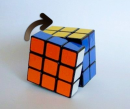
\includegraphics[width=.12\textwidth]{../graphics/moves/F.png} &
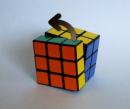
\includegraphics[width=.12\textwidth]{../graphics/moves/F_inv.png} &
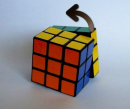
\includegraphics[width=.12\textwidth]{../graphics/moves/B.png} &
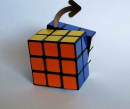
\includegraphics[width=.12\textwidth]{../graphics/moves/B_inv.png} &
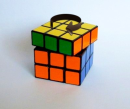
\includegraphics[width=.12\textwidth]{../graphics/moves/U.png} &
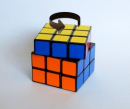
\includegraphics[width=.12\textwidth]{../graphics/moves/U_inv.png} \\
F & F' & B & B' & U & U' \\
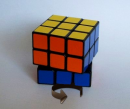
\includegraphics[width=.12\textwidth]{../graphics/moves/D.png} &
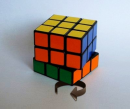
\includegraphics[width=.12\textwidth]{../graphics/moves/D_inv.png} &
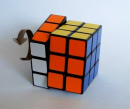
\includegraphics[width=.12\textwidth]{../graphics/moves/L.png} &
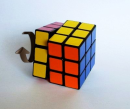
\includegraphics[width=.12\textwidth]{../graphics/moves/L_inv.png} &
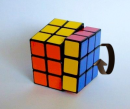
\includegraphics[width=.12\textwidth]{../graphics/moves/R.png} &
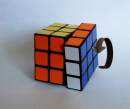
\includegraphics[width=.12\textwidth]{../graphics/moves/R_inv.png} \\
D & D' & L & L' & R & R' \\
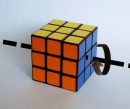
\includegraphics[width=.12\textwidth]{../graphics/moves/X.png} &
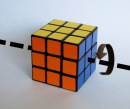
\includegraphics[width=.12\textwidth]{../graphics/moves/X_inv.png} &
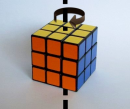
\includegraphics[width=.12\textwidth]{../graphics/moves/Y.png} &
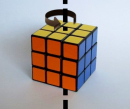
\includegraphics[width=.12\textwidth]{../graphics/moves/Y_inv.png} &
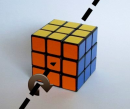
\includegraphics[width=.12\textwidth]{../graphics/moves/Z.png} &
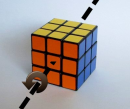
\includegraphics[width=.12\textwidth]{../graphics/moves/Z_inv.png} \\
X & X' & Y & Y' & Z & Z'
\end{tabular}
\end{table}
\end{frame}

\begin{frame}
\frametitle{Il nostro modello}
\begin{itemize}
\item Il cubo è memorizzato in un oggetto \texttt{RubikCubeModel}
\item Ogni faccia è memorizzata in un array $2\times 2$; le righe/colonne sono
numerate dall'alto verso il basso e da sinistra a destra (supponendo che il
solutore abbia la faccia di fronte)
\item \texttt{getSide} determina la faccia che in tale momento ha il colore dato
\item \texttt{getFace} recupera il colore di una facelet
\item Altri metodi autoesplicativi: \texttt{get3DEdge} (per gli angoli),
\texttt{get3DEdgeFacelet} (facelet di un angolo), \texttt{getCorner},
\texttt{getCornerFacelet}
\item Metodi \texttt{rotate*} per ruotare il cubo
\item Test standard: \texttt{isInStandardConfiguration},
\texttt{isWithSaneColors}, \texttt{isSolved}, \texttt{isCornerInPlace},
\texttt{isCornerInPlaceMaybeFlipped}, \texttt{isEdgeInPlace},
\texttt{isEdgeInPlaceMaybeFlipped}
\end{itemize}
\end{frame}

\begin{frame}[fragile]
\frametitle{Mosse di Singmaster}
\begin{itemize}
\item Sono state implementate le mosse standard di Singmaster
\item Ogni mossa (per motivi di astrazione) è una sottoclasse di \texttt{Move}
\item Il costruttore accetta come parametri il modello del cubo (in modo che il
cubo originale rimanga inalterato) e un parametro \texttt{reversed} (per sapere
se la mossa è diretta o inversa)
\item Per applicare una mossa, basta crearla e chiamare
\texttt{perform}/\texttt{reverse}:
\begin{center}
\begin{lstlisting}
(new B(m, reversed)).perform();
\end{lstlisting}
\end{center}
\item Ogni mossa genera un evento per comunicare i cambiamenti all'interfaccia
\end{itemize}
\end{frame}

\begin{frame}
\frametitle{Strategie di risoluzione}
\begin{itemize}
\item Sono sottoclassi di \texttt{ResolutionStrategy}
\item Accettano un cubo (\texttt{RubikCubeModel}) e restituiscono una lista di
mosse da eseguire per risolvere il problema (\texttt{getNextMoves})
\end{itemize}
\end{frame}

\begin{frame}
\frametitle{Pathfinding}
\begin{itemize}
\item Possiamo rappresentare i possibili svolgimenti di una partita con un
grafo i cui nodi sono la configurazione del cubo in un dato momento; due nodi
sono collegati se e solo se ci si può recare da una configurazione a un'altra
con una sola mossa
\item L'idea alla base della maggior parte degli algoritmi di risoluzione del
cubo è quella di trovare un cammino su tale albero avente origine nella radice
(configurazione iniziale) e termini nel cubo risolto
\end{itemize}
\end{frame}

\begin{frame}
\frametitle{A*}
\begin{itemize}
\item Mantengo due liste: una \emph{(open list)} che contiene i nodi ancora da
valutare, un'altra \emph{(closed list)} per i nodi già valutati
\item Fisso una funzione \emph{costo} per ogni nodo: esso deve essere,
intuitivamente, tanto minore quanto minore è il ``disordine'' rispetto al cubo
risolto
\item Calcolo per ogni nodo un indice
\[
f(n) = g(n) + h(n)
\]
dove $g(n)$ è il costo minimo dei nodi nella closed list e $h(n)$ è una stima
del costo del nodo $n$
\item A ogni passo sposto il nodo considerato dalla open alla closed list (ad
eccezione del caso in cui $g(n)$ diminuisca) e genero i suoi successori
(tenendo traccia di tale legame)
\item Al termine, estraendo il nodo con il minimo $f(n)$ e seguendo i genitori
ho la sequenza di mosse cercata (al contrario)
\end{itemize}
\end{frame}

\begin{frame}
\frametitle{IDA*}
\begin{itemize}
\item A* ha un difetto: richiede di esplorare tutto l'albero
\item Non fattibile per il cubo di Rubik (x configurazioni possibili!)
\item Basta non analizzare i rami per cui non crediamo di ottenere risultati
\item IDA* fa questo: per ogni nodo, se $f(n)$ è maggiore di un certo valore
limite che fissiamo, pota il ramo
\end{itemize}
\end{frame}

\begin{frame}
\frametitle{Fissare un'euristica}
Rimane solo un problema: fissare un'euristica $h(n)$ sufficientemente buona per
i nostri scopi
\end{frame}

\begin{frame}
\frametitle{L'algoritmo di Thistletwaite}
\begin{itemize}
\item Thistletwaite nel xxxx scoprì che era possibile dividere le mosse in
quattro gruppi:
\begin{align*}
1 & 2 \\
\end{align*}
\item Si noti che ogni gruppo è chiaramente incluso nel precedente e che 
l'ultimo gruppo comprende il cubo risolto
\item Idea: portare il cubo da una configurazione risolubile con tutte le mosse 
possibili (primo gruppo) in una risolubile solamente con mosse appartenenti al
secondo gruppo, quindi al terzo\dots
\item Esaminando le configurazioni possibili si può ricavare un buon 
coefficiente euristico FIXME cosa pesa di più?
\end{itemize}
\end{frame}

\begin{frame}
\frametitle{L'algoritmo a due fasi di Kociemba}
\end{frame}

\begin{frame}
\frametitle{L'algoritmo di Singmaster}
\end{frame}
\end{document}
